%*----------- SLIDE -------------------------------------------------------------
\begin{frame}[t]{Por que?}
    \transdissolve[duration=0.5]

    O problema consiste em:
    %\newline
    \begin{columns}[t]
        \column{.05\linewidth}
        \column{.4\linewidth}
        \begin{enumerate}
            \item Encerramento de um linha de pesquisa;
            \item paralisação da pesquisa em veículos aéreos;
            \item necessidade do desenvolvimento de competências.
        \end{enumerate}
        \column{.6\linewidth}
        \begin{center}
            %\centerline{
            \begin{figure}
                %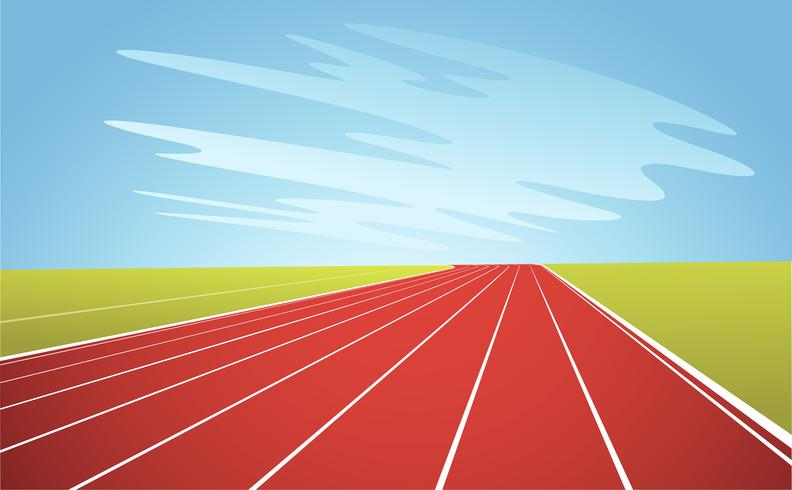
\includegraphics[width=1\textwidth]{pista}
                \caption{Pista de corrida \cite{agostini2007}}
                \roundpic[xshift=0cm,yshift=0cm]{2.5cm}{6cm}{pista}
                %\caption{Pista de corrida \cite{agostini2007}}
            \end{figure}
            %}
        \end{center}
    \end{columns}
    %*----------- notes
    \note[item]{Notes can help you to remember important information. Turn on the notes option.}
\end{frame}
%-
%*----------- SLIDE -------------------------------------------------------------
\begin{frame}[t]{Para resolver esse problema}
    \transdissolve[duration=0.5]

    Criação de um drone para o laboratório
    \newline
    \begin{columns}[t]
        \column{.6\linewidth}
        \begin{center}
            %\centerline{
            \begin{figure}
                %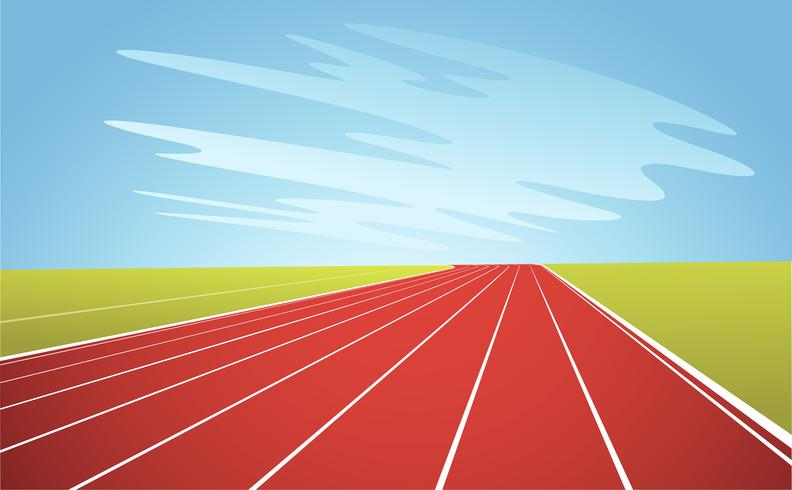
\includegraphics[width=1\textwidth]{pista}
                \caption{Pista de corrida \cite{agostini2007}}
                \roundpic[xshift=0cm,yshift=0cm]{2.5cm}{6cm}{pista}
                %\caption{Pista de corrida \cite{agostini2007}}
            \end{figure}
            %}
        \end{center}
    \end{columns}
    %*----------- notes
    \note[item]{Notes can help you to remember important information. Turn on the notes option.}
\end{frame}

%*----------- SLIDE -------------------------------------------------------------
\begin{frame}[t]{Estimativa de orçamento}
    \transboxout[duration=0.5]
%    \framesubtitle{Materiais necessários}
    \centering

    \begin{tabular}{ c|c|c|c }
      Peça                         & Quant. & Valor uni. &   Total    \\ \hline
      Helices                      &   4    &  R\$70.00  & R\$280.00  \\
      Motores Brushless (12V)      &   4    & R\$120.00  & R\$480.00  \\
      Controlador ESC              &   4    &  R\$80.00  & R\$320.00  \\
      Barometro                    &   1    & R\$100.00  & R\$100.00  \\
      IMU / MPU                    &   1    &  R\$30.00  &  R\$30.00  \\
      Laser unidirecional          &   1    & R\$100.00  & R\$100.00  \\
      Teensy microcontroller       &   1    & R\$400.00  & R\$400.00  \\
      Receptor de rádio + Controle &   1    & R\$620.00  & R\$620.00  \\
      Adaptador Wi-Fi              &   1    & R\$100.00  & R\$100.00  \\
      Estrutura de fibra           &   1    & R\$350.00  & R\$350.00  \\
      Bateria de Lipo              &   2    & R\$250.00  & R\$500.00  \\
      Power Hub                    &   1    & R\$100.00  & R\$100.00  \\ \hline
                                   &        &            & R\$3380.00
    \end{tabular}

    %*----------- notes
    \note[item]{Notes can help you to remember important information. Turn on the notes option.}
\end{frame}
%-
%*----------- SLIDE -------------------------------------------------------------
\begin{frame}[t]{Peças disponíveis (no lab)}
  \transboxout[duration=0.5]
%  \framesubtitle{Materiais necessarios}
  \centering
  \vfill

  \begin{tabular}{c | c }
              Peça            & Quant. \\ \hline
    Mint eye (câmera estéreo) & 1      \\
             Câmeras          & 2      \\
        Sensor Ultrassom      & 5      \\
           Jetson Nano        & 1
  \end{tabular}

  \vfill
  %*----------- notes
  \note[item]{Notes can help you to remember important information. Turn on the notes option.}
\end{frame}


%*----------- SLIDE -------------------------------------------------------------
\begin{frame}[c]{Darwin-OP - overview}
    %\transboxin[duration=1,direction=30]
    \centering

    \includemedia[
        width=0.7\linewidth,
        totalheight=0.39375\linewidth,
        activate=pageopen,
        passcontext,
        addresource=./Source/movies/Darwin-OP.mp4,
        flashvars={
                source=./Source/movies/Darwin-OP.mp4
                &autoPlay=true
                &Loop=false}
    ]{\fbox{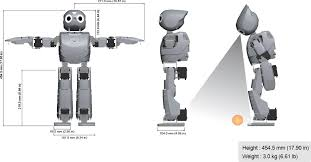
\includegraphics{darwin-op}}}{VPlayer.swf}

    %*----------- notes
    \note[item]{Notes can help you to remember important information. Turn on the notes option.}
\end{frame}
%-
%*----------- SLIDE -------------------------------------------------------------
\begin{frame}[t]{O sistema robótico}
    \transboxout[duration=0.5]
    \framesubtitle{Darwin-OP}
    \begin{columns}
        \column{.1\textwidth}
        \column{.4\textwidth}
        \column{.4\textwidth}
    \end{columns}

    \begin{block}{Um bloco de destaque}
        Um exemplo de block.\\
        Oferece um certo destaque.
    \end{block}

    \begin{alertblock}{Um bloco de destaque}
        Um exemplo de alertblock.\\
        Oferece um certo destaque.
    \end{alertblock}

    \begin{exampleblock}{Um bloco de destaque}
        Um exemplo de exampleblock.
    \end{exampleblock}
    %*----------- notes
    \note[item]{Notes can help you to remember important information. Turn on the notes option.}
\end{frame}
%-
%*----------- SLIDE -------------------------------------------------------------
\begin{frame}[t]{O sistema robótico}
    \transboxout[duration=0.5]
    \framesubtitle{PlantUML}

    \tikzstyle{every node}=[draw=black,thick,anchor=west]
    \tikzstyle{selected}=[draw=red,fill=red!30]
    \tikzstyle{optional}=[dashed,fill=gray!50]

    \begin{tikzpicture}[%
            grow via three points={one child at (0.5,-0.7) and
                    two children at (0.5,-0.7) and (0.5,-1.4)},
            edge from parent path={(\tikzparentnode.south) |- (\tikzchildnode.west)}]
        \node {texmf}
        child { node {doc}}
        child { node {fonts}}
        child { node {source}}
        child { node [selected] {tex}
                child { node {generic}}
                child { node [optional] {latex}}
                child { node {plain}}
            }
        child [missing] {}
        child [missing] {}
        child [missing] {}
        child { node {texdoc}};
    \end{tikzpicture}

    %*----------- notes
    \note[item]{Notes can help you to remember important information. Turn on the notes option.}
\end{frame}
%-
%*----------- SLIDE -------------------------------------------------------------
\begin{frame}[t]{O sistema robótico}
    \transboxout[duration=0.5]
    \framesubtitle{PlantUML}

    % Define block styles
    \tikzstyle{decision} = [diamond, draw, fill=blue!20,
    text width=4.5em, text badly centered, node distance=3cm, inner sep=0pt]
    \tikzstyle{block} = [rectangle, draw, fill=blue!20,
    text width=5em, text centered, rounded corners, minimum height=4em]
    \tikzstyle{line} = [draw, -latex']
    \tikzstyle{cloud} = [draw, ellipse,fill=red!20, node distance=3cm,
    minimum height=2em]

    \begin{tikzpicture}[node distance = 2cm, auto]
        % Place nodes
        \node [block] (init) {initialize model};
        \node [cloud, left of=init] (expert) {expert};
        \node [cloud, right of=init] (system) {system};
        \node [block, below of=init] (identify) {identify candidate models};
        \node [block, below of=identify] (evaluate) {evaluate candidate models};
        \node [block, left of=evaluate, node distance=3cm] (update) {update model};
        \node [decision, below of=evaluate] (decide) {is best candidate better?};
        \node [block, below of=decide, node distance=3cm] (stop) {stop};
        % Draw edges
        \path [line] (init) -- (identify);
        \path [line] (identify) -- (evaluate);
        \path [line] (evaluate) -- (decide);
        \path [line] (decide) -| node [near start] {yes} (update);
        \path [line] (update) |- (identify);
        \path [line] (decide) -- node {no}(stop);
        \path [line,dashed] (expert) -- (init);
        \path [line,dashed] (system) -- (init);
        \path [line,dashed] (system) |- (evaluate);
    \end{tikzpicture}

    %*----------- notes
    \note[item]{Notes can help you to remember important information. Turn on the notes option.}
\end{frame}
%-
%*----------- SLIDE -------------------------------------------------------------
\begin{frame}[t]{O sistema robótico}
    \transboxout[duration=0.5]
    \framesubtitle{PlantUML}

    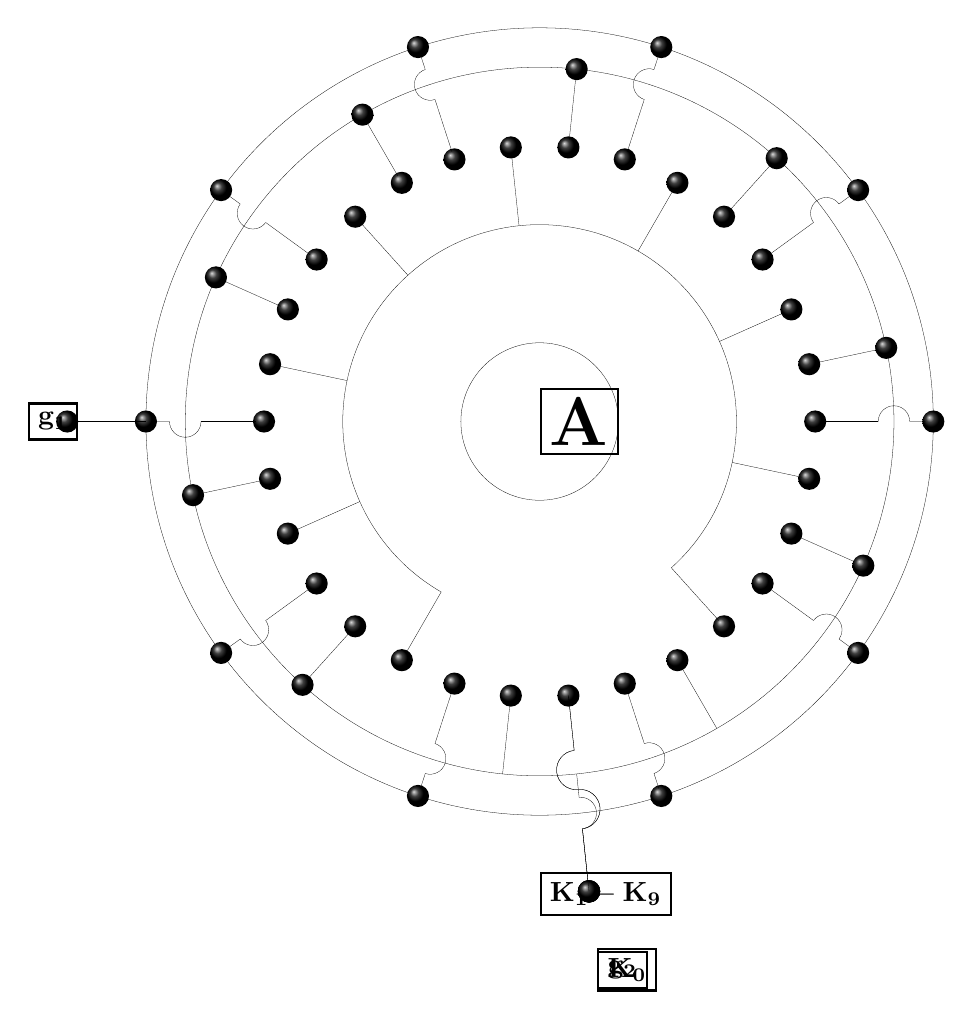
\begin{tikzpicture}[line width=0.1pt]
        \draw(0,0) circle(5cm);
        \draw(0,0) circle(1cm);
        \draw(0,0) node {\Huge$\mathbf{A}$};
        \draw(0,0) circle(4.5cm);
        \draw(-48:2.5) arc(-48:240:2.5cm);
        %% The outer nodes
        \foreach \x in {36,72,...,360}
        \shade[ball color=black](\x:5) circle(4pt);
        \foreach \nodes in {12,24,...,360}
        \shade[ball color=black](\nodes:3.5) circle(4pt);
        %%% The connecting nodes
        \foreach \angle in {-48,-12,...,240}
        \draw(\angle:2.5) --++(\angle:0.9cm);
        %%% outer interconnects
        \foreach \angle in {-24,12,...,306}
        \draw(\angle:3.6) --++(\angle:0.9cm);
        \foreach \y in {-24,12,...,240}
        \shade[ball color=black](\y:4.5cm) circle(4pt);

        %% outer most connections
        \foreach \angle in{-36,0,...,306}
        \draw(\angle:4.9cm) --(\angle:4.7cm) [rotate=\angle]arc(0:180:0.20cm);
        \foreach \angle in{-36,0,...,306}
        \draw(\angle:4.3cm) --(\angle:3.6cm);
        %% Outer connects and leads
        \shade[ball color=black](276:6) circle(4pt);
        \draw(276:6)circle(4pt)--(276:5.2)[rotate=276]arc(0:180:0.25cm);
        \draw(276:7)node {$\mathbf{K_0}$};
        \draw(276:4.2)[rotate=276]arc(180:360:0.25cm);
        \draw(276:4.2)--(276:3.5);

        %% Exploitation of circular symmetry of the required figure

        {[rotate=72]
        \shade[ball color=black](276:6) circle(4pt);
        \draw(276:6)circle(4pt)--(276:5.2)[rotate=276]arc(0:180:0.25cm);
        \draw(270:6)node {$\mathbf{K_1-K_9}$};
        \draw(276:4.2)[rotate=276]arc(180:360:0.25cm);%%%
        \draw(276:4.2)--(276:3.5);
        }

        {[rotate=-48]
        \shade[ball color=black](276:6) circle(4pt);
        \draw(276:6)circle(4pt)--(276:5.2)[rotate=276]arc(0:180:0.20cm);
        \draw(276:7)node {$\mathbf{g_2}$};
        \draw(276:4.8)--(276:4.5);
        }

        \draw(180:5)--(180:6);
        \shade[ball color=black](180:6) circle(4pt);
        \draw(180:6.5)node{$\mathbf{g_1}$};
    \end{tikzpicture}

    %*----------- notes
    \note[item]{Notes can help you to remember important information. Turn on the notes option.}
\end{frame}
%-
